\section{\sysname{}}
\label{sec:system}

In contrast to existing approaches that require developers to specify the
concrete policies, \sysname{} uses a special operator \texttt{maybe} to express
structured adaptation. The specifications are hints on potential operations
without exact quantifications. \sysname{} then automatically learns concrete
degradation strategies (the profile) using profiling data (either offline or
online) and controls the application execution at runtime. The profiles also
have additional benefits such as coordination among competing streaming
flows. \autoref{fig:overview} provides an overview of the systems (in three
stages) and we describe each stage in turn.

\begin{figure}
  \centering
  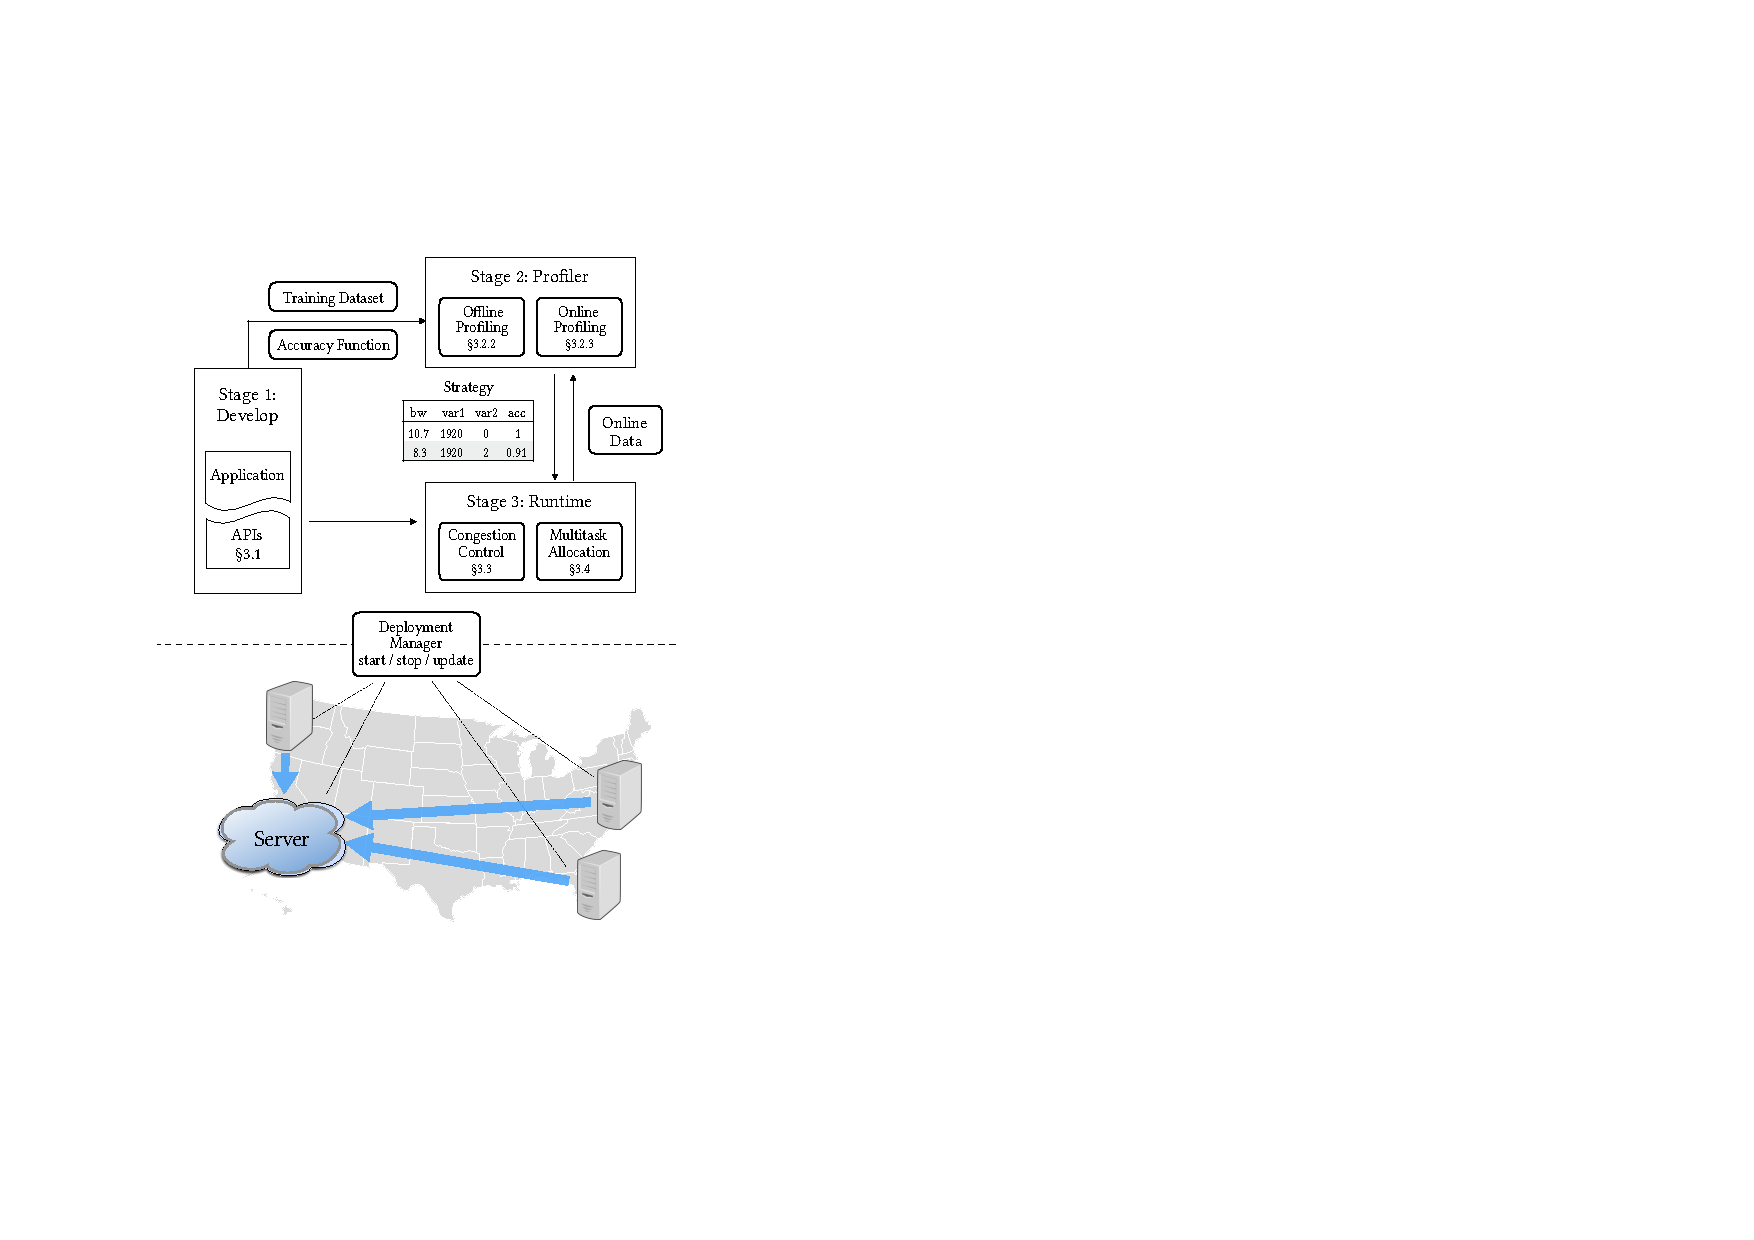
\includegraphics[width=.9\linewidth]{figures/system.pdf}
  \caption{\sysname{} overview and components.}
  \label{fig:overview}
\end{figure}

\subsection{APIs for Structured Adaptation}
\label{sec:struct-adapt}

%% Introduce graphs of operators model
The vast majority of stream processing applications today are constructed as a
directed graph of operators~\cite{toshniwal2014storm, zaharia2013discretized}).
\sysname{} employs such a programming model that integration with existing
applications will require minimal effort. \autoref{tab:operators} lists a few
example operators that \sysname{} supports.

In this model, each operator transforms existing streams into new
streams. Operators are specializable by user-defined functions (UDF). Optionally
developers can provide objects that implement a callable interface. Such objects
can be used to hold application states.

\begin{table*}
  \centering
  \begin{tabular}{ c r l }
    \toprule
    \multirow{7}{*}{Normal Operators}
    & \textit{map} (f: I $\Rightarrow$ O) & Stream<I> $\Rightarrow$ Stream<O> \\
    & \textit{filter} (f: I $\Rightarrow$ bool) & Stream<I> $\Rightarrow$
                                                 Stream<I> \\
    & \textit{skip} n(i: Integer) & Stream<I> $\Rightarrow$ Stream<I> \\
    & \textit{sliding\_window} (count: Integer, f: Vec<I> $\Rightarrow$ O) & Stream<I> $\Rightarrow$
                                                                            Stream<O> \\
    & \textit{tumbling\_window} (count: Integer, f: Vec<I> $\Rightarrow$ O) & Stream<I> $\Rightarrow$
                                                                             Stream<O> \\
    & \textit{timed\_window} (time: Duration, f: Vec<I> $\Rightarrow$ O) & Stream<I> $\Rightarrow$
                                                                          Stream<O> \\
    & ... & ... \\
    \midrule
    \multirow{4}{*}{Degradation Operators}
    & \textit{maybe} (knobs: Vec<T>, f:  (T, I) $\Rightarrow$ I) & Stream<I> $\Rightarrow$
                                                                 Stream<I> \\
    & \textit{maybe\_skip} (knobs: Vec<Integer>) & Stream<I> $\Rightarrow$ Stream<I> \\
    & \textit{maybe\_downsample} (knobs: Vec<(Integer, Interger)>) & Stream<Image> $\Rightarrow$ Stream<Image> \\
    & ... & ... \\
    \bottomrule
  \end{tabular}
  \caption{A comparison between normal stream processing operators and our
    degradation operators. \texttt{Vec<T>} represents a list of elements of type
    T. \texttt{Option<T>} indicates an optional element of type T which is
    either present \texttt{Some(T)} or absent \texttt{None}.}
  \label{tab:operators}
\end{table*}

\sysname{} offers a special operator \texttt{maybe} to annotate degradation
operations. Developers use \texttt{maybe} with concrete operations that affect
the data size as well as data fidelity: these are the knobs tunable by the
system to explore performance trade-offs. The basic form of \texttt{maybe}
operator takes two arguments: a knob and a function. The knob is a vector of
values with type $T$ that encodes possible levels of degradation. The function
performs the actual operation. By default, the function needs to satisfy the
type constrain: $f(T, I) \Rightarrow I$. That is, only operations that does not
alter the type of the data stream are allowed. In this way, downstream operators
can work without the need to know if the degradation is in effect or not. A
relaxed version, \texttt{maybe\_with\_default}, exists for flexibility; but care
should be taken to use.

We illustrate the idea of \texttt{maybe} operator with an example that quantizes
a stream of integers in the Rust programming language. One possible
implementation is as follows:

\begin{lstlisting}
    let quantized_stream = vec![1, 2, 3, 4].into_stream()
        .maybe(vec![2, 4], |k, p| p.wrapping_div(k));
        .collect();
\end{lstlisting}

The code creates a stream of integers [1, 2, 3, 4] and pass it through a
degradation operation. In this example, the knob is chosen as [2, 4]. The
degradation function performs a wrapping (modular) division where the divisor is
the knob. Depending on the quantization level, the output will be either [1, 2,
3, 4] (no degradation), [0, 1, 1, 2] (k=2), or [0, 0, 0, 1] (k=4). The
\texttt{collect} method will run this stream and hold the output in a vector.
If the stream is subsequently encoded (e.g. run-length encoding as in
JPEG~\cite{wallace1992jpeg}) for transmission, the data size will change
according to the level of degradation.

Based on the \texttt{maybe} primitive, one can implement wrappers for common
degradation operations. For example, \texttt{maybe\_skip} will optionally
subsample a stream; and \texttt{maybe\_downsample} can adjust the image
resolution to a configured target. \sysname{} provides a few such operations as
libraries for developers.

Using our APIs, the example mentioned in \autoref{sec:manual-policy} can now be
implemented as follows:

\begin{lstlisting}
   let app = Camera::new((1920, 1080, 30))
      .maybe_downsample(vec![(1600, 900), (1280, 720)])
      .maybe_skip(vec![2, 5])
      .map(|frame| frame.show())
      .compose();
\end{lstlisting}

This snippet first instantiate a \texttt{Camera} source, which produces
\texttt{Stream<Image>} with 1920x1080 resolution and 30 FPS. Two degradation
operations are chained after the source: one that downsample the resolution to
either 1600x900 or 1280x720; the other skip the frame with a parameter of 2 or
5, resulting in 30/(2+1)=10 FPS or 30/(5+1)= 6 FPS. After the degradation,
images are shown on the display. In practice, further processing (such as
encoding and transmission) operators can be chained.

While \maybe{} itself has simplified the specification of degradation, the exact
level of degradation has to be known for precise rate adjustment at runtime. The
second stage of \sysname{} performs automatic profiling.

\subsection{Automatic Profiling}
\label{sec:automatic-profiling}

The goal of the profiling is to learn how different levels of degradation
affects the bandwidth demand and application accuracy. By exploring this
trade-off space, \sysname{} generates a Pareto-optimal \textit{profile} for each
application. We formulate the profiling and discuss the designs for offline and
online profiling.

\subsubsection{Profiling Formalism and Offline Profiling}
\label{sec:formalize-profiling}

Suppose in a stream processing application that $n$ \maybe{} operators are
used. Each introduces a knob $k_i$. We assume these operators are independent
from each other; their combination forms a \textit{configuration}
$c = [k_{1}, k_{2}, ... k_{n}]$. The set of all possible configurations
$\mathbb{C}$ is the space that our profiling system needs to explore. For each
configuration $c$, there are two mappings that our system needs to explore: a
mapping from $c$ to its bandwidth requirement $B(c)$ and its accuracy measure
$A(c)$. \autoref{tab:notations} summarizes the symbols used in this paper.

The Pareto-optimal set $\mathbb{P}$ is then defined (\autoref{eq:pareto}): for
all $c \in \mathbb{P}$, there is no alternative configuration $c'$ that requires
less bandwidth while giving a higher accuracy.

{\small
\begin{equation}
  \mathbb{P} = \{ c \in \mathbb{C} : \{ c' \in \mathbb{C}: B(c') < B(c),
  A(c') > A(c) \} = \varnothing\}
  \label{eq:pareto}
\end{equation}
}%

\begin{table}
  \centering
  \begin{tabular}{r l}
    \toprule
    \textbf{Symbol} & \textbf{Description} \\
    \midrule
    $n$ & number of degradation operations \\
    $k_i$ & the \textit{i}-th degradation knob \\
    $c = [k_{1}, k_{2}, ... k_{n}]$ & one specific configuration \\
    $\mathbb{C}$ & the set of all configurations \\
    \midrule
    $B(c)$ & bandwidth requirement for $c$ \\
    $A(c)$ & accuracy measure for $c$ \\
    $\mathbb{P}$ & Pareto efficienct set \\
    \bottomrule
  \end{tabular}
  \caption{Notations used in profiling.}
  \label{tab:notations}
\end{table}

Since there is often no closed form relation for $B(c)$ and $A(c)$, our system
takes a data-driven approach: with a representative training dataset and an
application-specific utility function, our system evaluates each configuration
for its bandwidth and accuracy. The accuracy can either be measured against the
groundtruth; or in the case when labelled dataset is not available, \sysname{}
uses the results when all degradations are turned off as the reference.

The profiling is expensive, because all possible configurations come from a
combinatorial space of all knobs. When there is no a prior information about
each configuration's impact, only an exhaustive search can find the optimal set.
When done at \textit{offline}, the time required is accepted. However, this
prohibits us from doing profiling naively at online.

\subsubsection{Online Profiling}
\label{sec:online-profiling}

While the offline profiling generates one strategy based on the training data,
the strategy is susceptible to a problem known as ``model drift''. When the
required bandwidth is underestimated, data will be queued at the sender and
application latency will increase. When the accuracy is incorrectly measured,
the actual application performance will be suboptimal. The drift needs to be
corrected online.

There are two particular challenges for online profiling.

The first is the lack of groundtruth data or reference data. During the online
execution, it's often infeasible to get labelled data as the groundtruth. For
example, image labelling is known to be labor intensive and time
consuming~\cite{russell2008labelme}. In addition, the original un-degraded data
need to be transmitted from the sender.  \sysname{} addresses labelling by using
the un-degraded data as the reference and allocate additional bandwidth for
backhaulling portions of the un-degraded data. While the additional bandwidth
seems a waste, in our design, during the runtime's probing phase, the original
data can enjoy a free ride. Details of the probing is in \autoref{sec:runtime}.

The second challenge is how to profile efficiently. Naively profiling every
configuration as the offline profiler does does not warrant a timely update. We
use the offline profiling information as a prior to speed-up the online
profiler. Specficially, we employ two techniques: degradation-aware
parallelization and partial profiling.

\para{Degradation-aware parallelization:} The profiling tasks of exploring all
configurations are easily parallelizable. Normal job schedulers don't assume the
knowledge of estimated task completion time, therefore the parallel execution
suffers from sub-optimal assignments. Aided with the offline profiling
statistics (the time it requires to profile a particular configuration), we can
schedule the online profiling tasks with a longest first scheduling that
minimizes the makespan.

\para{Partial profiling:} In time domain, the profiling could use a smaller
chunk of data to approximate the best strategy. Besides, we can profiling a
subset of the total configurations and measures its difference from the current
profile. If the difference exceeds a certain threshold, it triggers a full
profiling.

\subsection{Runtime Adaptation}
\label{sec:runtime}

\begin{figure}
  \centering
  \resizebox{\columnwidth}{!}{
    \begin{tikzpicture}
  %
  % Define basic styles
  %
  % Node
  \tikzstyle{module} = [draw, very thick, rounded corners,
  fill=white, minimum height=2.5em, inner sep=0.5em,
  rectangle, font={\bfseries}, align=center]
  \tikzstyle{cmodule} = [module, fill=black!20]

  % Edge
  \tikzstyle{stateEdgePortion} = [black, thick];
  \tikzstyle{dataEdge} = [stateEdgePortion, ->];
  \tikzstyle{controlEdgePartial} = [stateEdgePortion, dashed];
  \tikzstyle{controlEdge} = [controlEdgePartial, ->];
  \tikzstyle{controlDoubleEdge} = [controlEdgePartial, <->];
  \tikzstyle{edgeLabel} = [pos=0.5, text centered, font={\itshape}];

  \node[name=client, draw, very thick, fill=white,
  double copy shadow={shadow xshift=2pt, shadow yshift=-2pt, fill=white, draw},
  text height=13em, text width=31.5em] {};

  \node[name=server, draw, very thick, fill=white, draw,
  right=of client.north east, anchor=north west, xshift=1em,
  text height=7em, text width=12.5em] {};

  \node[module, name=source, below right=of client.north west,
  xshift=-1.5em, yshift=1.5em] {Source};
  \node[module, name=transform, right of=source, xshift=3.5em] {Transform};
  \node[cmodule, name=degrade, right of=transform, xshift=3.7em] {Degrade};
  \node[cmodule, name=queue, right of=degrade, xshift=3em] {Queue};
  \node[cmodule, name=socket, right of=queue, xshift=3em, text width=3em] {Socket};
  \node[cmodule, name=receiver, right of=socket, xshift=7em] {Receiver};
  \node[module, name=analytics, right of=receiver, xshift=3em] {Analytics};

  \node[cmodule, name=cc, at=($(queue)!0.5!(socket)$), yshift=-6em]
  {Congestion\\Controller};

  \draw ($(source.east)$) edge[dataEdge] ($(transform.west)$);
  \draw ($(transform.east)$) edge[dataEdge] ($(degrade.west)$);
  \draw ($(degrade.east)$) edge[dataEdge] ($(queue.west)$);
  \draw ($(queue.east)$) edge[dataEdge] ($(socket.west)$);
  \draw ($(socket.east)$) edge[dataEdge] node[edgeLabel, yshift=0.6em] {data}
  ($(receiver.west)$);
  \draw ($(receiver.east)$) edge[dataEdge] ($(analytics.west)$);

  %% Control path
  \draw let
  \p1 = ($(cc.center)$), \p2 = ($(degrade.center)$)
  in ($(cc.west)$) edge[controlEdgePartial] (\x2, \y1)
  (\x2, \y1) edge[controlEdge] ($(degrade.south)$);

  \draw let
  \p1 = ($(queue.south)$), \p2 = ($(cc.north)$)
  in ($(\x1, \y1) + (1em,0)$) edge[controlEdge] ($(\x1, \y2) + (1em,0)$);

  \draw let
  \p1 = ($(socket.south)$), \p2 = ($(cc.north)$)
  in ($(\x1, \y1) + (-1em,0)$) edge[controlDoubleEdge] ($(\x1, \y2) + (-1em,0)$);

  \node[name=clientlabel, above right=of client.south west, xshift=-2em, yshift=-2em] {Edge (Client)};
  \node[name=clientlabel, above left=of server.south east, xshift=2em, yshift=-2em] {Server};

  %%
  %% Legend
  %%
  \node[name=datalegend, below=1.5em of server.south west, xshift=2em]
  {\small Data Plane};
  \draw ($(datalegend.west) + (-2em, 0)$) edge[dataEdge]
  ($(datalegend.west) + (-0.5em, 0)$);

  \node[name=controllegend, below=2.5em of datalegend.west, anchor=west]
  {\small Control Plane};
  \draw ($(controllegend.west) + (-2em, 0)$) edge[controlEdge]
  ($(controllegend.west) + (-0.5em, 0)$);

  \node[name=applegend, right=3em of datalegend.east]
  {\small Application Logic};
  \node[module, name=applegendbox, left=0.1em of applegend, text width=0.3em,
  minimum height=0em] {};

  \node[name=syslegend, below=2.5em of applegend.west, anchor=west]
  {\small Runtime};
  \node[cmodule, name=syslegendbox, left=0.1em of syslegend, text width=0.3em,
  minimum size=0em] {};

\end{tikzpicture}

%%% Local Variables:
%%% mode: latex
%%% TeX-master: "sosp17"
%%% End:

  }
  % \includegraphics[width=\linewidth]{figures/runtime-adaptation.pdf}
  \caption{Runtime adaptation system architecture. The grey components are what
    \sysname{} provides.}
  \label{fig:runtime}
\end{figure}

At runtime, the user program is automatically converted to a client half and
server half; and \sysname{} abstracts the communication as well as rate
adaptation (\autoref{fig:runtime}).

The data source with degradation is a module that supports \texttt{update}
function. To handle insufficient bandwidth, an object-level queue bridges data
generation (source) and the network IO. Followed by the queue is a socket module
that abstracts the network communication. It transmits data as fast as possible
and also supports traffic probing. The growth of the queue indicates congestions
and will trigger the congestion controller. The socket module estimates actual
available bandwidth. To avoid spikes in the bandwidth measurement, exponential
smoothing is employed.

At the core of our rate adjustment is a congestion control algorithms assisted
with stream data generation rate (\autoref{fig:cc}).

\para{Startup behavior:} When the application starts up, it performs its first
(and most rapid) rate increase. On each \texttt{Q.NoQueue} received, it
decreases the level of degradation, hence an increase of the data rate.

\para{Reacting to congestion:} When congestion is detected by an increase of the
queued item, TCP's send rate is used as an approximation of the bottleneck
bandwidth of the current connection. \sysname{} then adjusts the level of
degradation such that the expected data rate is below the estimated bandwidth
(often with a factor to allow the queue draining). After the queue is drained
and there is no queued item for a configurable period, it fires
\texttt{Q.NoQueue} event to the congestion controller, which then enters into
the \texttt{Steady} state.

\para{Steady state:} The steady state is the ideal state that the streaming
application should stay in. If currently the application is operating at the
maximum rate, then there is no need to probe. However, we might be in steady
state with degradation, in this case, we need to probe to test if there is more
bandwidth. Enter probe state.

\para{Probe for available bandwidth:} In contrast to BBR that adjusts the pace
of transmission, our probe is to send dummy traffic. If the application is
configured to run online profiling, then the probe traffic is the raw data.

% \begin{figure}
%   \centering
%   \resizebox{\columnwidth}{!}{
%     \begin{tikzpicture}[
  state/.style = { draw, very thick, fill=white, rounded corners=1em,
    minimum height=3em, minimum width=7em, node distance=7em, font={\bfseries},
    align=center },
  edge portion/.style = { black, thick },
  transition/.style = { edge portion, -> },
  algorithm/.style = { draw, thin, fill=white },
  ]

  \node [state] (startup) {
    STARTUP };
  \node [state] (congestion) [right=of startup] {CONGESTION};
  \draw [transition] (startup) -- (congestion)
  node [midway, auto] {Q.Congestion};

  \node [state] (steady) [below=of congestion] {STEADY};

  \draw [transition] ($(congestion.south west)!0.4!(congestion.south east)$)
  to node[midway, sloped, below] {Q.NoQueue}
  ($(steady.north west)!0.4!(steady.north east)$);

  \draw [transition] ($(steady.north west)!0.6!(steady.north east)$)
  to node[midway, sloped, below] {Q.Congestion}
  ($(congestion.south west)!0.6!(congestion.south east)$);

  \node [state] (probe) [left=of steady] {PROBE};

  \draw [transition] ($(steady.south west)!0.6!(steady.north west)$)
  -- ($(probe.south east)!0.6!(probe.north east)$)
  node[midway, auto, swap] {Q.Probe};

  \draw [transition, <-] ($(steady.south west)!0.4!(steady.north west)$)
  -- ($(probe.south east)!0.4!(probe.north east)$)
  node[midway, auto, align=left] {Q.Congestion | \\ IO.ProbeDone};

\end{tikzpicture}


%%% Local Variables:
%%% mode: latex
%%% TeX-master: "sosp17"
%%% End:

%   }
%   \caption{Congestion Control Algorithm}
%   \label{fig:cc}
% \end{figure}

\begin{figure}
  \centering
  \includegraphics[width=\columnwidth]{figures/cc.pdf}
  \caption{Congestion Control Algorithm}
  \label{fig:cc}
\end{figure}

%%% Local Variables:
%%% mode: latex
%%% TeX-master: "sosp17"
%%% End:

\subsection{Multitask Adaptation}
\label{sec:multitask-adaptation}

Briefly discuss the issues without coordination.

\newpage

%%% Local Variables:
%%% mode: latex
%%% TeX-master: "sosp17"
%%% End:


%%% Local Variables:
%%% mode: latex
%%% TeX-master: "sosp17"
%%% End:
